% ==========================================================================
%  SPHERExLens -- presentation deck (Beamer, 16:9, LuaLaTeX)
%  Content: paper/slides_and_script.pdf (30 slides)
%  Build:   lualatex spherexlens_beamer.tex   (twice)
% ==========================================================================
\documentclass[aspectratio=169,10pt]{beamer}

\usepackage{fontspec}
% Lato: clean vertical metrics and a professional humanist sans.
\setsansfont{Lato}
\setmainfont{Lato}
\setmonofont{DejaVu Sans Mono}[Scale=0.88]

\usepackage{amsmath,amssymb}
\usepackage{xcolor}
\usepackage{tikz}
\usetikzlibrary{arrows.meta,positioning,calc,fit,backgrounds,shapes.geometric,
  decorations.pathreplacing,patterns}
\usepackage{pgfplots}
\pgfplotsset{compat=1.18}
\usepackage{adjustbox}
\usepackage{booktabs}
\usepackage{array}

% ------------------------------------------------------------------ colours
\definecolor{ink}{HTML}{14213A}
\definecolor{slate}{HTML}{3F4A5A}
\definecolor{muted}{HTML}{6E7A8A}
\definecolor{accent}{HTML}{1F6FB2}
\definecolor{accent2}{HTML}{E8F1F8}
\definecolor{good}{HTML}{1E7B4F}
\definecolor{good2}{HTML}{E7F3EC}
\definecolor{bad}{HTML}{B3261E}
\definecolor{bad2}{HTML}{FAECEA}
\definecolor{warn}{HTML}{8A5A00}
\definecolor{warn2}{HTML}{FBF3E2}
\definecolor{rule}{HTML}{D5DAE2}
\definecolor{purple}{HTML}{6D28D9}
\definecolor{purple2}{HTML}{F3E8FF}
\definecolor{paper}{HTML}{F8F5F2}

% ------------------------------------------------------------------- chrome
\usetheme{default}
\usecolortheme{default}
\setbeamertemplate{navigation symbols}{}
\setbeamercolor{normal text}{fg=ink,bg=paper}
\setbeamercolor{structure}{fg=accent}
\setbeamercolor{itemize item}{fg=accent}
\setbeamercolor{itemize subitem}{fg=muted}

\setbeamerfont{frametitle}{size=\fontsize{15.6}{18.4},series=\bfseries}
\setbeamerfont{itemize/enumerate body}{size=\fontsize{9.2}{12.6}}
\setbeamerfont{itemize/enumerate subbody}{size=\fontsize{8.4}{11.4}}
\setbeamersize{text margin left=7.5mm,text margin right=7.5mm}
\raggedright

% kicker, drawn above the title
\newcommand{\kickertext}{}
\newcommand{\kicker}[1]{\renewcommand{\kickertext}{#1}}
\setbeamertemplate{headline}{%
  \vspace*{3.0mm}%
  \hspace*{7.5mm}%
  \begin{minipage}{\dimexpr\paperwidth-15mm\relax}%
    {\fontsize{6.3}{7.6}\selectfont\color{muted}%
      \addfontfeature{LetterSpace=15}\MakeUppercase{\kickertext}}%
    \hfill{\fontsize{6.3}{7.6}\selectfont\color{muted}%
      \addfontfeature{LetterSpace=15}\MakeUppercase{SPHERExLens \,·\, SPHEREx DR1}}%
    \par\vspace{1.0mm}%
    {\color{rule}\rule{\linewidth}{0.35pt}}%
  \end{minipage}%
  \vspace{0.5mm}%
}

% page number + progress rule, drawn below the body
\setbeamertemplate{footline}{%
  \hbox{%
    \begin{minipage}{\paperwidth}%
      \hspace*{7.5mm}%
      \begin{minipage}{\dimexpr\paperwidth-15mm\relax}%
        {\color{rule}\rule{\linewidth}{0.9pt}}\par\vspace{0.9mm}%
        {\fontsize{6.2}{7.2}\selectfont\color{muted}%
          \insertframenumber\,/\,\inserttotalframenumber\hfill SPHERExLens \;\textbullet\; finding what changed}%
      \end{minipage}%
    \end{minipage}}%
  \vspace{1.6mm}%
}


% ------------------------------------------------------------------ macros
% Cards are built from \colorbox + minipage: predictable height, no package
% interaction with beamer, and they can sit inside a column.
\newcommand{\panel}[3][2.2mm]{% [pad] {background} {content}
  \begingroup\setlength{\fboxsep}{#1}\setlength{\fboxrule}{0pt}%
  \noindent\colorbox{#2}{\begin{minipage}{\dimexpr\linewidth-2\fboxsep\relax}%
    \vspace{0.15mm}#3\end{minipage}}\par\endgroup}

\newcommand{\lead}[1]{%
  \panel[2.2mm]{accent2}{\fontsize{9.4}{12.2}\selectfont\color{ink}#1}\vspace{1.0mm}}

\newcommand{\callout}[2]{%
  \panel[2.1mm]{#1!9!white}{\fontsize{7.7}{9.7}\selectfont\color{ink}#2}}

\newcommand{\figcap}[1]{%
  \par\vspace{0.6mm}{\fontsize{6.6}{8.0}\selectfont\color{muted}#1\par}}

% Graphics are taller than a text line, so the pinned baseline grid is relaxed
% around them; otherwise TeX would let the picture overlap the line above.
\newcommand{\figureblock}[1]{%
  \par\vspace{1.4mm}%
  \begingroup\lineskiplimit=0pt\lineskip=2.5pt\relax
    \begin{center}#1\end{center}%
  \endgroup\par\vspace{0.4mm}}

\newcommand{\kpi}[3]{%
  \begingroup\setlength{\fboxsep}{1.8mm}\setlength{\fboxrule}{0pt}%
  \noindent\colorbox{#1!9!white}{\begin{minipage}{\dimexpr\linewidth-2\fboxsep\relax}%
    \centering{\fontsize{13.5}{14.5}\selectfont\bfseries\color{#1}#2\par}%
    \vspace{0.2mm}{\fontsize{7.1}{8.4}\selectfont\color{ink}#3\par}%
  \end{minipage}}\par\endgroup}

\newcommand{\chip}[2]{%
  {\setlength{\fboxsep}{1.0mm}\colorbox{#1!12!white}{%
    \fontsize{6.3}{7.2}\selectfont\color{#1}\textbf{#2}}}}

% two columns: #1 = left width, #2 left, #3 right
\newcommand{\twocol}[3]{% #1 = left width in cm (frame text width is 14.5cm)
  \noindent\begin{minipage}[t]{#1}\vspace{0pt}#2\end{minipage}\hfill
  \begin{minipage}[t]{\dimexpr14.5cm-#1-0.55cm\relax}\vspace{0pt}#3\end{minipage}\par}

% frame title: title + short accent rule
\setbeamertemplate{frametitle}{%
  \vspace{0.6mm}%
  {\usebeamerfont{frametitle}\color{ink}\raggedright\insertframetitle\par}%
  \vspace{0.8mm}{\color{accent}\rule{16mm}{1.4pt}}\par\vspace{1.2mm}%
}

\setlength{\parindent}{0pt}
\setlength{\parskip}{0pt}
\newcommand{\code}[1]{{\ttfamily\fontsize{8.6}{10}\selectfont\color{ink!88!black}#1}}
\newcommand{\arcsec}{\ensuremath{{}^{\prime\prime}}}
\newcommand{\arcmin}{\ensuremath{{}^{\prime}}}

\begin{document}
\renewcommand{\inserttotalframenumber}{30}
\begin{frame}[plain]
\vspace{3mm}
\noindent
\begin{minipage}[c]{9.0cm}
  {\fontsize{6.6}{8}\selectfont\color{muted}\addfontfeature{LetterSpace=17}%
   NASA/IPAC IRSA · SPHEREx DATA RELEASE 1\par}
  \vspace{4mm}
  {\fontsize{26}{29}\selectfont\bfseries\color{ink}Finding What Changed\par}
  \vspace{2mm}
  {\fontsize{11}{14}\selectfont\color{slate}%
   A difference-imaging and transient-discovery pipeline for the SPHEREx
   all-sky infrared survey\par}
  \vspace{4mm}
  {\color{accent}\rule{24mm}{2pt}}\par
  \vspace{3.4mm}
  {\fontsize{8.6}{11.2}\selectfont\color{slate}%
   \textbf{18} fields \;·\; \textbf{246} cutouts \;·\; \textbf{109} detections \;·\;
   \textbf{99} explained \;·\; \textbf{10} candidates\par}
  \vspace{5mm}
  {\fontsize{8}{10}\selectfont\color{muted}%
   Evan Lim \quad·\quad November 2026 \quad·\quad 21-minute talk\par}
\end{minipage}\hfill
\begin{minipage}[c]{4.9cm}
  \centering
  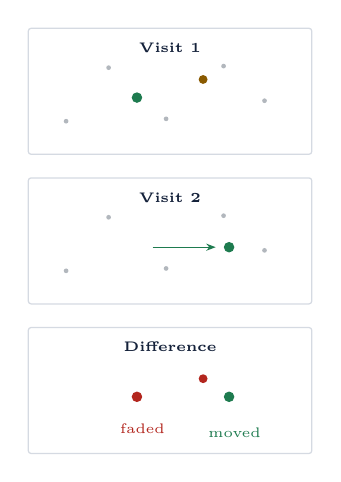
\begin{tikzpicture}[font=\fontsize{5.2}{6.2}\selectfont]
    \foreach \dy/\lab in {0/{Visit 1},-1.90/{Visit 2},-3.80/{Difference}}{
      \draw[rule,line width=0.45pt,fill=white,rounded corners=1pt]
        (0,\dy) rectangle (3.6,\dy+1.60);
      \node[text=ink,font=\fontsize{5.4}{6.4}\selectfont\bfseries,anchor=north]
        at (1.8,\dy+1.54) {\lab};
    }
    \foreach \x/\y in {0.48/0.42,1.02/1.10,1.75/0.45,2.48/1.12,3.00/0.68}{
      \fill[slate!40] (\x,\y) circle (0.85pt);}
    \fill[good] (1.38,0.72) circle (1.9pt);
    \fill[warn] (2.22,0.95) circle (1.6pt);
    \foreach \x/\y in {0.48/0.42,1.02/1.10,1.75/0.45,2.48/1.12,3.00/0.68}{
      \fill[slate!40] (\x,\y-1.90) circle (0.85pt);}
    \fill[good] (2.55,0.72-1.90) circle (1.9pt);
    \draw[-{Stealth[length=1.2mm]},good,line width=0.5pt]
      (1.58,0.72-1.90) -- (2.38,0.72-1.90);
    \fill[bad] (1.38,0.72-3.80) circle (1.9pt);
    \fill[good] (2.55,0.72-3.80) circle (1.9pt);
    \fill[bad] (2.22,0.95-3.80) circle (1.6pt);
    \node[text=good,font=\fontsize{4.6}{5.6}\selectfont,anchor=north]
      at (2.62,0.45-3.80) {moved};
    \node[text=bad,font=\fontsize{4.6}{5.6}\selectfont,anchor=north]
      at (1.45,0.50-3.80) {faded};
  \end{tikzpicture}
\end{minipage}
\end{frame}

\begin{frame}
\kicker{Why this is hard}
\frametitle{Two visits reveal what one image cannot.}
\lead{A second visit six months later turns a photograph into a measurement of change.}

\begin{itemize}\setlength{\itemsep}{0.4mm}
  \item Subtract the two visits and the stationary sky cancels to zero.
  \item What survives is a \textbf{dipole} (the source moved) or a \textbf{monopole}
        (it brightened or faded).
  \item Instrumental systematics outnumber the real events, so the detector has to be
        calibrated rather than trusted.
\end{itemize}

\figureblock{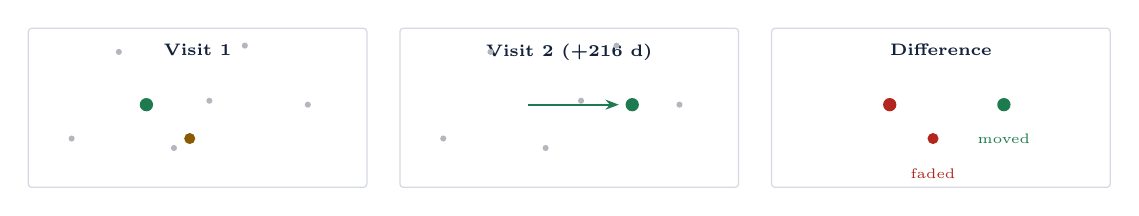
\begin{tikzpicture}[font=\fontsize{5.4}{6.4}\selectfont]
  \foreach \i/\lab in {0/{Visit 1},1/{Visit 2 (+216 d)},2/{Difference}}{
    \draw[rule,line width=0.45pt,fill=white,rounded corners=1.2pt]
      (\i*4.72,0) rectangle (\i*4.72+4.30,2.02);
    \node[text=ink,font=\fontsize{6.2}{7.2}\selectfont\bfseries,anchor=north]
      at (\i*4.72+2.15,1.95) {\lab};
  }
  % stationary sky
  \foreach \x/\y in {0.55/0.62,1.15/1.72,1.85/0.50,2.75/1.80,3.55/1.05,2.30/1.10}{
    \fill[slate!40] (\x,\y) circle (1.1pt);
    \fill[slate!40] (\x+4.72,\y) circle (1.1pt);
  }
  % mover and fader in epoch 1
  \fill[good] (1.50,1.05) circle (2.4pt);
  \fill[warn] (2.05,0.62) circle (2.0pt);
  % epoch 2
  \fill[good] (4.72+2.95,1.05) circle (2.4pt);
  \draw[-{Stealth[length=1.7mm]},good,line width=0.6pt]
    (4.72+1.62,1.05) -- (4.72+2.78,1.05);
  % difference
  \fill[bad] (9.44+1.50,1.05) circle (2.4pt);
  \fill[good] (9.44+2.95,1.05) circle (2.4pt);
  \fill[bad] (9.44+2.05,0.62) circle (2.0pt);
  \node[text=good,font=\fontsize{5.2}{6.2}\selectfont,anchor=north]
    at (9.44+2.95,0.80) {moved};
  \node[text=bad,font=\fontsize{5.2}{6.2}\selectfont,anchor=north]
    at (9.44+2.05,0.36) {faded};
\end{tikzpicture}
\figcap{The stationary sky subtracts to zero, so only motion or a flux change survives.
Green = positive, red = negative, grey = unchanged sky.}
}
\end{frame}

\begin{frame}
\kicker{The task, stated precisely}
\frametitle{What the pipeline has to output}
\lead{Given two visits to a 9-arcminute field, produce a defensible list of candidate changes —
each with a position, a significance, a shape and an identity.}

\twocol{7.2cm}{%
  \begin{itemize}\setlength{\itemsep}{0.5mm}
    \item \textbf{Input:} 180×180 pixel cut-outs, variance planes and a 32-bit quality mask.
    \item \textbf{Rule:} keep every pixel whose significance exceeds $6\sigma$ — 109 detections
          over 18 fields.
    \item \textbf{Output:} each detection is attributed before it can be called a candidate.
  \end{itemize}
}{%
  \centering
  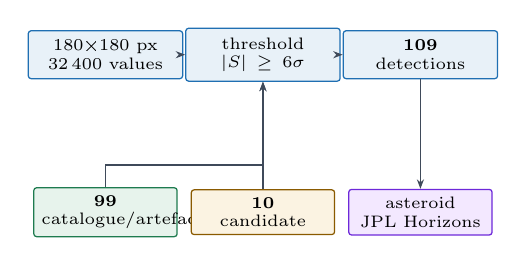
\begin{tikzpicture}[font=\fontsize{5.6}{6.6}\selectfont,
    bx/.style={draw=accent,line width=0.45pt,fill=accent2,rounded corners=1pt,
      align=center,inner sep=1.2mm,text width=1.72cm},
    ar/.style={-{Stealth[length=1.2mm]},draw=slate,line width=0.45pt}]
    \node[bx] (in) at (0.95,2.55) {180×180 px\\ 32\,400 values};
    \node[bx] (th) at (2.95,2.55) {threshold\\ $|S|\ge 6\sigma$};
    \node[bx] (cd) at (4.95,2.55) {\textbf{109}\\ detections};
    \node[draw=good,line width=0.45pt,fill=good2,rounded corners=1pt,
      align=center,inner sep=1mm,text width=1.62cm] (kn) at (0.95,0.55)
      {\textbf{99}\\ catalogue/artefact};
    \node[draw=warn,line width=0.45pt,fill=warn2,rounded corners=1pt,
      align=center,inner sep=1mm,text width=1.62cm] (ca) at (2.95,0.55)
      {\textbf{10}\\ candidate};
    \node[draw=purple,line width=0.45pt,fill=purple2,rounded corners=1pt,
      align=center,inner sep=1mm,text width=1.62cm] (as) at (4.95,0.55)
      {asteroid\\ JPL Horizons};
    \draw[ar] (in) -- (th); \draw[ar] (th) -- (cd);
    \draw[ar] (cd.south) -- (as.north);
    \draw[ar] (kn.north) -- ++(0,0.28) -| (th.south);
    \draw[ar] (ca.north) -- ++(0,0.28) -| (th.south);
  \end{tikzpicture}
  \figcap{Every pixel becomes a verdict. A change is reported only after a catalogue, an
  asteroid or an artefact is ruled out.}
}
\end{frame}

\begin{frame}
\kicker{Four questions, four answers}
\frametitle{What the project set out to measure}
\vspace{0.4mm}
\noindent
\begin{minipage}[t]{3.42cm}
  \kpi{accent}{$S\sim\mathcal{N}(0,1)$?}{Calibration}
  \vspace{0.6mm}{\fontsize{7.4}{9.4}\selectfont\color{ink}Robust MAD scaling makes the map
  unit-variance on real co-adds.}
\end{minipage}\hfill
\begin{minipage}[t]{3.42cm}
  \kpi{good}{dipole vs monopole}{Morphology}
  \vspace{0.6mm}{\fontsize{7.4}{9.4}\selectfont\color{ink}Separable at $3\arcsec$ once pairing
  is bounded by physical motion.}
\end{minipage}\hfill
\begin{minipage}[t]{3.42cm}
  \kpi{warn}{91\%}{Identity}
  \vspace{0.6mm}{\fontsize{7.4}{9.4}\selectfont\color{ink}99 of 109 detections are explained by
  Gaia, WISE, VSX or NEOWISE.}
\end{minipage}\hfill
\begin{minipage}[t]{3.42cm}
  \kpi{purple}{69.3\%}{Completeness}
  \vspace{0.6mm}{\fontsize{7.4}{9.4}\selectfont\color{ink}Strict recovery over 12\,240 injected
  sources; it was 0.2\% before v2.}
\end{minipage}

\vspace{2.6mm}
\figureblock{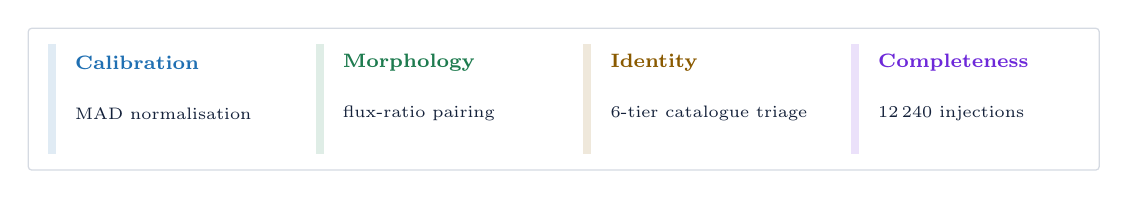
\begin{tikzpicture}[font=\fontsize{6.4}{7.6}\selectfont]
  \draw[rule,line width=0.45pt,fill=white,rounded corners=1.2pt] (0,0) rectangle (13.6,1.80);
  \foreach \x/\txt/\col in {0.25/{Calibration}/accent, 3.65/{Morphology}/good,
                            7.05/{Identity}/warn, 10.45/{Completeness}/purple}{
    \fill[\col!14] (\x,0.20) rectangle (\x+0.10,1.60);
    \node[anchor=west,text=\col,font=\fontsize{6.8}{8}\selectfont\bfseries] at (\x+0.22,1.36) {\txt};
  }
  \node[anchor=west,text=ink,font=\fontsize{6.2}{7.4}\selectfont] at (0.47,0.72) {MAD normalisation};
  \node[anchor=west,text=ink,font=\fontsize{6.2}{7.4}\selectfont] at (3.87,0.72) {flux-ratio pairing};
  \node[anchor=west,text=ink,font=\fontsize{6.2}{7.4}\selectfont] at (7.27,0.72) {6-tier catalogue triage};
  \node[anchor=west,text=ink,font=\fontsize{6.2}{7.4}\selectfont] at (10.67,0.72) {12\,240 injections};
\end{tikzpicture}
\figcap{The four questions map onto four measurable outputs — and each has a number attached
in this deck.}}
\end{frame}

\begin{frame}
\kicker{Prior art · image subtraction}
\frametitle{Forty years of subtracting one image from another}
\lead{Every survey that looks twice needs a way to cancel the sky.}

\figureblock{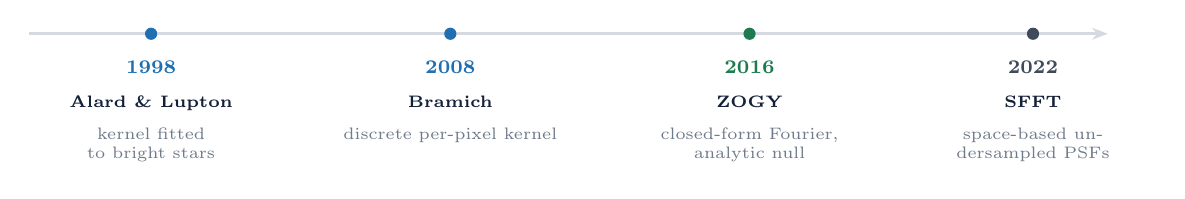
\begin{tikzpicture}[font=\fontsize{6.2}{7.4}\selectfont]
  \draw[-{Stealth[length=2mm]},draw=rule,line width=1pt] (0,1.62) -- (13.7,1.62);
  \foreach \x/\yr/\nm/\desc/\col in {
      1.55/1998/{Alard \& Lupton}/{kernel fitted to bright stars}/accent,
      5.35/2008/{Bramich}/{discrete per-pixel kernel}/accent,
      9.15/2016/{ZOGY}/{closed-form Fourier, analytic null}/good,
      12.75/2022/{SFFT}/{space-based undersampled PSFs}/slate}{
    \fill[\col] (\x,1.62) circle (2.2pt);
    \node[anchor=north,text=\col,font=\fontsize{7.4}{8.6}\selectfont\bfseries] at (\x,1.40) {\yr};
    \node[anchor=north,text=ink,font=\fontsize{6.4}{7.6}\selectfont\bfseries] at (\x,0.95) {\nm};
    \node[anchor=north,text=muted,font=\fontsize{5.8}{7}\selectfont,text width=2.9cm,align=center]
      at (\x,0.55) {\desc};
  }
\end{tikzpicture}
\figcap{Two families: a fitted kernel (1998–2008), then a closed-form solution (2016–2022).}}

\vspace{0.2mm}
\begin{itemize}\setlength{\itemsep}{0.3mm}
  \item Fitting a kernel needs isolated bright stars — exactly what crowded fields lack.
  \item ZOGY convolves each image with the other's PSF, so nothing is fitted, and the null is
        Gaussian wherever the sky is constant.
\end{itemize}
\end{frame}

\begin{frame}
\kicker{Prior art · brokers and vetoes}
\frametitle{Every survey does the same four things}
\lead{Detection is rarely the bottleneck; vetoing is.}

\figureblock{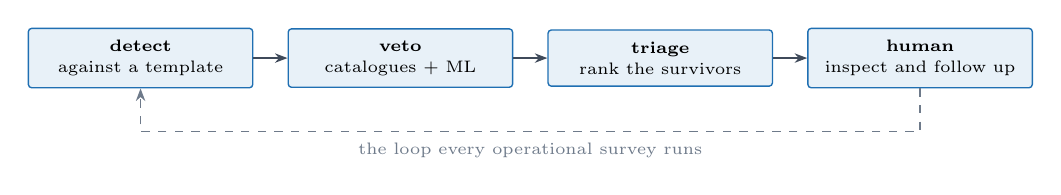
\begin{tikzpicture}[font=\fontsize{6.4}{7.6}\selectfont,
  b/.style={draw=accent,line width=0.5pt,fill=accent2,rounded corners=1.2pt,
    align=center,inner sep=1.5mm,text width=2.55cm},
  ar/.style={-{Stealth[length=1.6mm]},draw=slate,line width=0.5pt}]
  \node[b] (d) at (1.55,1.35) {\textbf{detect}\\ against a template};
  \node[b] (v) at (4.85,1.35) {\textbf{veto}\\ catalogues + ML};
  \node[b] (t) at (8.15,1.35) {\textbf{triage}\\ rank the survivors};
  \node[b] (h) at (11.45,1.35) {\textbf{human}\\ inspect and follow up};
  \draw[ar] (d) -- (v); \draw[ar] (v) -- (t); \draw[ar] (t) -- (h);
  \draw[ar,dashed,draw=muted] (h.south) -- ++(0,-0.55) -| (d.south);
  \node[text=muted,font=\fontsize{5.8}{7}\selectfont] at (6.5,0.18)
    {the loop every operational survey runs};
\end{tikzpicture}
\figcap{ANTARES, ALeRCE, Lasair and Fink run this loop for optical surveys; none publishes an
end-to-end instance for SPHEREx.}}

\vspace{0.2mm}
\begin{itemize}\setlength{\itemsep}{0.3mm}
  \item Brokers ingest \emph{already-detected} alerts; the pixels and the subtraction stay inside
        the survey.
  \item The gap is not an algorithm — it is a reproducible, auditable instance built only from
        public data.
\end{itemize}
\end{frame}

\begin{frame}
\kicker{The instrument}
\frametitle{Six arrays, 102 bands, one sweep every six months}
\lead{Each cut-out is a small stamp from a 70\,MB frame, and carries its own quality data.}

\figureblock{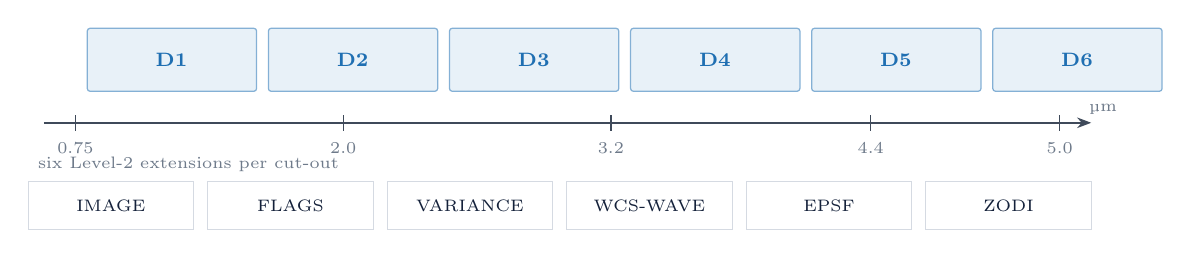
\begin{tikzpicture}[font=\fontsize{6}{7.2}\selectfont]
  \draw[-{Stealth[length=1.8mm]},draw=slate,line width=0.6pt] (0.2,1.55) -- (13.5,1.55);
  \foreach \x/\lab in {0.6/0.75, 4.0/2.0, 7.4/3.2, 10.7/4.4, 13.1/5.0}{
    \draw[slate,line width=0.5pt] (\x,1.45) -- (\x,1.65);
    \node[anchor=north,text=muted,font=\fontsize{5.6}{6.8}\selectfont] at (\x,1.42) {\lab};
  }
  \node[anchor=west,text=muted,font=\fontsize{5.8}{7}\selectfont] at (13.35,1.72) {µm};
  \foreach \lab/\x in {D1/0.75, D2/3.05, D3/5.35, D4/7.65, D5/9.95, D6/12.25}{
    \draw[draw=accent!55,fill=accent2,line width=0.45pt,rounded corners=1pt]
      (\x,1.95) rectangle (\x+2.15,2.75);
    \node[text=accent,font=\fontsize{6.6}{7.8}\selectfont\bfseries] at (\x+1.07,2.35) {\lab};
  }
  \foreach \i/\nm in {0/{IMAGE},1/{FLAGS},2/{VARIANCE},3/{WCS-WAVE},4/{EPSF},5/{ZODI}}{
    \draw[draw=rule,fill=white,line width=0.4pt] (\i*2.28,0.20) rectangle (\i*2.28+2.10,0.80);
    \node[text=ink,font=\fontsize{5.8}{7}\selectfont] at (\i*2.28+1.05,0.50) {\nm};
  }
  \node[anchor=west,text=muted,font=\fontsize{5.6}{6.8}\selectfont] at (0.0,1.02)
    {six Level-2 extensions per cut-out};
\end{tikzpicture}
\figcap{Arrays D1–D6 tile 0.75–5.0\,µm; a linear variable filter puts a different wavelength on
each detector row, so every pixel has its own colour.}}

\vspace{0.2mm}
\begin{itemize}\setlength{\itemsep}{0.3mm}
  \item Six-month cadence: solar-system objects leave the field between visits, so survivors are
        genuine variability or motion.
  \item Live mode co-adds six arrays; archive mode falls back to D1 and D4 when a band is missing.
\end{itemize}
\end{frame}

\begin{frame}
\kicker{Data path}
\frametitle{Eighteen fields, fetched as 5\,MB stamps}
\lead{A 70\,MB parent frame is useless on a laptop, so the pipeline asks for small cut-outs.}

\twocol{7.4cm}{%
  \begin{itemize}\setlength{\itemsep}{0.4mm}
    \item Two paths to the same pixels: an SIA2 cone search, or a direct S3 read from the public
          \code{nasa-irsa-spherex} bucket.
    \item Every cut-out must keep a 12-pixel margin and stay under 50\% flagged, or it is refused.
    \item Five mandatory targets plus thirteen famous benchmarks — galaxies, nebulae, quasars and
          nearby stars.
  \end{itemize}
}{%
  \centering
  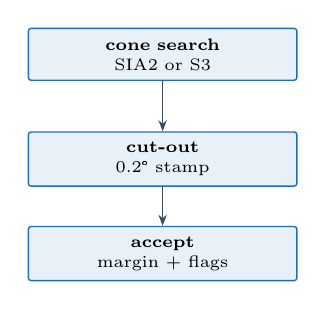
\begin{tikzpicture}[font=\fontsize{6}{7.2}\selectfont,
    b/.style={draw=accent,line width=0.5pt,fill=accent2,rounded corners=1pt,
      align=center,inner sep=1.3mm,text width=3.15cm},
    ar/.style={-{Stealth[length=1.4mm]},draw=slate,line width=0.5pt}]
    \node[b] (a) at (1.75,3.05) {\textbf{cone search}\\ SIA2 or S3};
    \node[b] (b) at (1.75,1.72) {\textbf{cut-out}\\ 0.2° stamp};
    \node[b] (c) at (1.75,0.52) {\textbf{accept}\\ margin + flags};
    \draw[ar] (a) -- (b); \draw[ar] (b) -- (c);
  \end{tikzpicture}
  \figcap{Metadata first, pixels second: a cone search returns the product list, then only the
  stamps that pass the acceptance test are downloaded.}
}
\end{frame}

\begin{frame}
\kicker{System design}
\frametitle{Seven subsystems, one science core}
\lead{The same code runs on a laptop, in a batch job and in the live web service.}

\figureblock{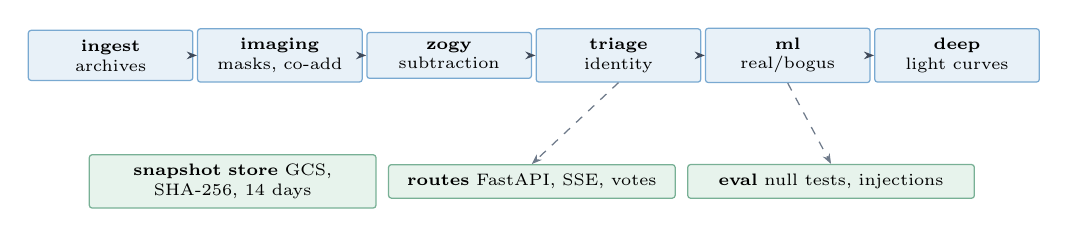
\begin{tikzpicture}[font=\fontsize{5.9}{7.1}\selectfont,
  b/.style={draw=accent!60,fill=accent2,line width=0.45pt,rounded corners=1pt,
    align=center,inner sep=1.2mm},
  ar/.style={-{Stealth[length=1.3mm]},draw=slate,line width=0.45pt}]
  \node[b,text width=1.85cm] (i) at (1.05,2.30) {\textbf{ingest}\\ archives};
  \node[b,text width=1.85cm] (m) at (3.20,2.30) {\textbf{imaging}\\ masks, co-add};
  \node[b,text width=1.85cm] (z) at (5.35,2.30) {\textbf{zogy}\\ subtraction};
  \node[b,text width=1.85cm] (t) at (7.50,2.30) {\textbf{triage}\\ identity};
  \node[b,text width=1.85cm] (l) at (9.65,2.30) {\textbf{ml}\\ real/bogus};
  \node[b,text width=1.85cm] (d) at (11.80,2.30) {\textbf{deep}\\ light curves};
  \draw[ar] (i) -- (m); \draw[ar] (m) -- (z); \draw[ar] (z) -- (t); \draw[ar] (t) -- (l);
  \draw[ar] (l) -- (d);
  \node[draw=good!60,fill=good2,line width=0.45pt,rounded corners=1pt,
    align=center,inner sep=1.2mm,text width=3.4cm] (s) at (2.6,0.70)
    {\textbf{snapshot store} GCS, SHA-256, 14 days};
  \node[draw=good!60,fill=good2,line width=0.45pt,rounded corners=1pt,
    align=center,inner sep=1.2mm,text width=3.4cm] (r) at (6.4,0.70)
    {\textbf{routes} FastAPI, SSE, votes};
  \node[draw=good!60,fill=good2,line width=0.45pt,rounded corners=1pt,
    align=center,inner sep=1.2mm,text width=3.4cm] (e) at (10.2,0.70)
    {\textbf{eval} null tests, injections};
  \draw[ar,dashed,draw=muted] (t.south) -- (r.north);
  \draw[ar,dashed,draw=muted] (l.south) -- (e.north);
\end{tikzpicture}
\figcap{Science stages above, serving layers below. All seven share one JSON detection contract,
so a batch result is byte-identical to a live one.}}

\vspace{0.2mm}
\begin{itemize}\setlength{\itemsep}{0.3mm}
  \item 21\,429 runtime Python lines; the contract (\code{CONTRACT.md}) is the interface between
        science and serving.
\end{itemize}
\end{frame}

\begin{frame}
\kicker{Resilience}
\frametitle{When an archive goes down, the pipeline does not stop}
\lead{Every external service is called behind a fallback, and every failure is reported rather
than hidden.}

\twocol{6.6cm}{%
  \begin{itemize}\setlength{\itemsep}{0.4mm}
    \item Gaia is queried through three mirrors in turn: IPAC, then STScI MAST, then CDS VizieR.
    \item Asteroids come from JPL Horizons, enriched by the Small-Body Database and cross-checked
          against CADC SSOIS.
    \item Optical confirmation comes from CSA NEOSSat, cleaned of darks and flats before use.
  \end{itemize}
}{%
  \centering
  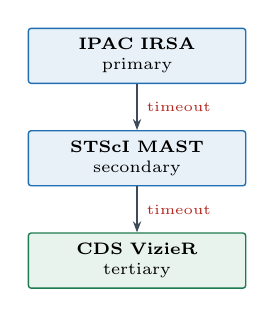
\begin{tikzpicture}[font=\fontsize{6}{7.2}\selectfont,
    b/.style={draw=accent,line width=0.5pt,fill=accent2,rounded corners=1pt,
      align=center,inner sep=1.3mm,text width=2.5cm},
    g/.style={draw=good,line width=0.5pt,fill=good2,rounded corners=1pt,
      align=center,inner sep=1.3mm,text width=2.5cm},
    ar/.style={-{Stealth[length=1.4mm]},draw=slate,line width=0.5pt}]
    \node[b] (a) at (1.55,3.25) {\textbf{IPAC IRSA}\\ primary};
    \node[b] (b) at (1.55,1.95) {\textbf{STScI MAST}\\ secondary};
    \node[g] (c) at (1.55,0.65) {\textbf{CDS VizieR}\\ tertiary};
    \draw[ar] (a) -- node[right,font=\fontsize{5.4}{6.6}\selectfont,text=bad] {timeout} (b);
    \draw[ar] (b) -- node[right,font=\fontsize{5.4}{6.6}\selectfont,text=bad] {timeout} (c);
  \end{tikzpicture}
  \figcap{Three tiers, two timeouts: a Gaia cross-match survives an outage at any mirror.}
}
\end{frame}

% ================================================ 10. MASKING & CO-ADD ===
\begin{frame}
\kicker{Theory I · preprocessing}
\frametitle{Fourteen defect bits go, two stay}
\lead{The quality mask decides what the difference image can ever contain.}

\twocol{6.8cm}{%
  \begin{itemize}\setlength{\itemsep}{0.4mm}
    \item Fourteen bits are rejected: cosmic rays, saturation, hot and cold pixels, persistence
          and outliers.
    \item Two bits are kept — \code{FULLSAMPLE} and \code{SOURCE} — because rejecting them erased
          real flux around bright stars.
    \item A pixel masked in epoch 2 is dropped in epoch 1 too, so a mask hole cannot fake a
          dipole.
  \end{itemize}
}{%
  \centering
  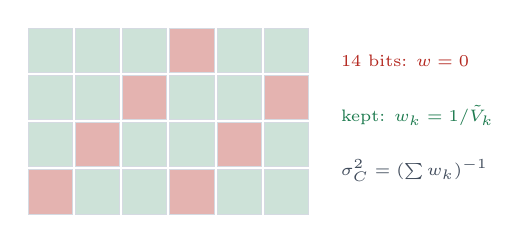
\begin{tikzpicture}[font=\fontsize{5.8}{7}\selectfont]
    \foreach \i in {0,...,5}{\foreach \j in {0,...,3}{
      \pgfmathsetmacro{\m}{int(mod(\i*7+\j*3,10))}
      \ifnum\m<3 \def\cc{bad!35}\else\def\cc{good!22}\fi
      \draw[rule,line width=0.3pt,fill=\cc]
        (\i*0.60,\j*0.60) rectangle (\i*0.60+0.56,\j*0.60+0.56);
    }}
    \node[anchor=west,text=bad] at (3.85,1.95) {14 bits: $w=0$};
    \node[anchor=west,text=good] at (3.85,1.25) {kept: $w_k=1/\tilde V_k$};
    \node[anchor=west,text=slate] at (3.85,0.55) {$\sigma_C^2=(\sum w_k)^{-1}$};
  \end{tikzpicture}
  \figcap{Inverse-variance stacking: bad pixels carry zero weight, kept pixels are weighted by
  their own variance.}
}
\end{frame}

\begin{frame}
\kicker{Theory II · proper subtraction}
\frametitle{Subtract in the Fourier domain, with nothing fitted}
\lead{ZOGY convolves each image with the other's PSF, then divides by the noise that survives.}

\figureblock{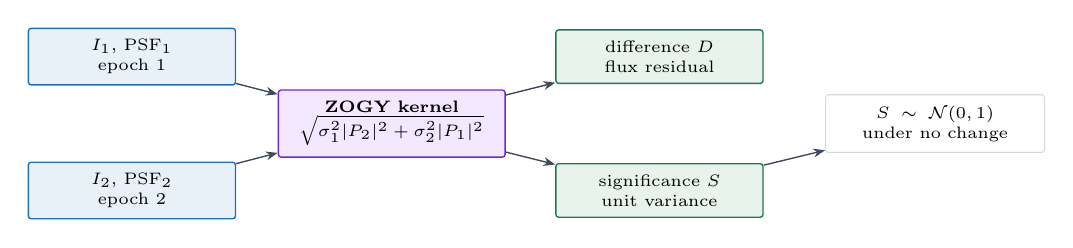
\begin{tikzpicture}[font=\fontsize{6}{7.2}\selectfont,
  b/.style={draw=accent,line width=0.5pt,fill=accent2,rounded corners=1pt,
    align=center,inner sep=1.4mm,text width=2.35cm},
  p/.style={draw=purple,line width=0.5pt,fill=purple2,rounded corners=1pt,
    align=center,inner sep=1.4mm,text width=2.6cm},
  g/.style={draw=good,line width=0.5pt,fill=good2,rounded corners=1pt,
    align=center,inner sep=1.4mm,text width=2.35cm},
  ar/.style={-{Stealth[length=1.5mm]},draw=slate,line width=0.5pt}]
  \node[b] (i1) at (1.35,2.55) {$I_1$, PSF$_1$\\ epoch 1};
  \node[b] (i2) at (1.35,0.85) {$I_2$, PSF$_2$\\ epoch 2};
  \node[p] (z)  at (4.65,1.70) {\textbf{ZOGY kernel}\\ $\sqrt{\sigma_1^2|P_2|^2+\sigma_2^2|P_1|^2}$};
  \node[g] (d)  at (8.05,2.55) {difference $D$\\ flux residual};
  \node[g] (s)  at (8.05,0.85) {significance $S$\\ unit variance};
  \node[draw=rule,fill=white,line width=0.4pt,rounded corners=1pt,
    align=center,inner sep=1.4mm,text width=2.5cm] (n) at (11.55,1.70)
    {$S\sim\mathcal{N}(0,1)$\\ under no change};
  \draw[ar] (i1) -- (z); \draw[ar] (i2) -- (z);
  \draw[ar] (z) -- (d); \draw[ar] (z) -- (s);
  \draw[ar] (s) -- (n);
\end{tikzpicture}
\figcap{Two 2-D FFTs per epoch pair — under 0.6\,s for a $180^2$ frame — and an analytic null that
makes the threshold a design choice, not a tuning knob.}}

\vspace{0.2mm}
\begin{itemize}\setlength{\itemsep}{0.3mm}
  \item Empirical PSFs come from a 21×21 zone grid, chosen by the cut-out's WCS coordinates.
\end{itemize}
\end{frame}

\begin{frame}
\kicker{Theory III · the threshold}
\frametitle{Why 6σ is a decision, not a habit}
\lead{Because the null is unit-variance Gaussian, the false-alarm budget can be computed before
looking at the data.}

\twocol{6.3cm}{%
  \centering
  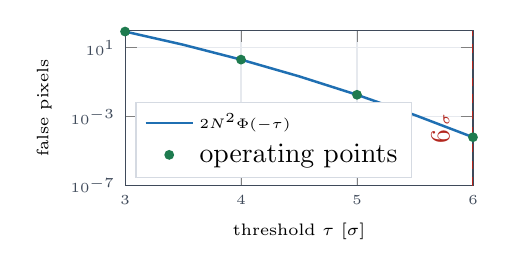
\begin{tikzpicture}[font=\fontsize{5.8}{7}\selectfont]
    \begin{axis}[width=6.0cm,height=3.55cm,xmin=3,xmax=6,ymin=1e-7,ymax=1e2,
      ymode=log,xlabel={threshold $\tau$ [$\sigma$]},xlabel style={font=\fontsize{5.6}{6.8}\selectfont},
      ylabel={false pixels},ylabel style={font=\fontsize{5.6}{6.8}\selectfont},
      tick label style={font=\fontsize{5.4}{6.6}\selectfont,text=slate},
      axis line style={slate},grid=major,grid style={rule!60},
      legend style={font=\fontsize{5}{6},draw=rule,at={(0.03,0.05)},anchor=south west},
      legend cell align=left]
      \addplot[accent,line width=0.9pt] coordinates {(3,87.5) (3.5,15.1) (4,2.05) (4.5,0.220) (5,0.0186) (5.5,0.00123) (6,6.4e-5)};
      \addlegendentry{$2N^2\Phi(-\tau)$}
      \addplot[only marks,mark=*,mark size=1.4pt,good,line width=0.7pt] coordinates {
        (3,87.5) (4,2.05) (5,0.0186) (6,6.4e-5)};
      \addlegendentry{operating points}
      \draw[bad,dashed,line width=0.7pt] (axis cs:6,1e-7) -- (axis cs:6,1e2);
      \node[text=bad,font=\fontsize{5}{6},rotate=90,anchor=south] at (axis cs:5.88,2e-4) {6\,$\sigma$};
    \end{axis}
  \end{tikzpicture}
}{%
  \begin{itemize}\setlength{\itemsep}{0.4mm}
    \item At $5\sigma$ the analytic budget is 0.0186 false pixels per frame — but the empirical
          null on real co-adds gave \textbf{0.86} false candidates per field.
    \item Raising the cut to $6\sigma$ halves that to \textbf{0.48} per field with no loss of
          strict recovery.
    \item Sky-correlated noise is not Gaussian, so the threshold is calibrated empirically.
  \end{itemize}
}
\end{frame}

% ================================================= 13. MORPHOLOGY =========
\begin{frame}
\kicker{Theory IV · what a change looks like}
\frametitle{Three shapes, three physical stories}
\lead{The geometry of the residual is the only clue to what actually happened.}

\figureblock{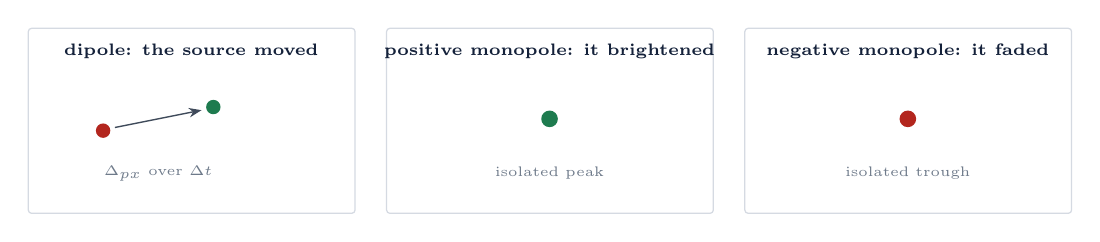
\begin{tikzpicture}[font=\fontsize{6}{7.2}\selectfont]
  \foreach \i/\lab in {0/{dipole: the source moved},1/{positive monopole: it brightened},
                       2/{negative monopole: it faded}}{
    \draw[rule,line width=0.45pt,fill=white,rounded corners=1.2pt]
      (\i*4.55,0) rectangle (\i*4.55+4.15,2.35);
    \node[text=ink,font=\fontsize{6.2}{7.4}\selectfont\bfseries,anchor=north]
      at (\i*4.55+2.07,2.27) {\lab};
  }
  % dipole
  \fill[bad] (0.95,1.05) circle (2.6pt);
  \fill[good] (2.35,1.35) circle (2.6pt);
  \draw[-{Stealth[length=1.6mm]},slate,line width=0.5pt] (1.10,1.09) -- (2.20,1.31);
  \node[text=muted,font=\fontsize{5.4}{6.6}\selectfont,anchor=north] at (1.65,0.72)
    {$\Delta_{px}$ over $\Delta t$};
  % positive
  \fill[good] (4.55+2.07,1.20) circle (3.0pt);
  \node[text=muted,font=\fontsize{5.4}{6.6}\selectfont,anchor=north] at (4.55+2.07,0.72)
    {isolated peak};
  % negative
  \fill[bad] (9.10+2.07,1.20) circle (3.0pt);
  \node[text=muted,font=\fontsize{5.4}{6.6}\selectfont,anchor=north] at (9.10+2.07,0.72)
    {isolated trough};
\end{tikzpicture}
\figcap{A dipole is a source that moved between visits; a lone peak is brightening; a lone trough
is fading or an eclipse. Pairing the lobes by physical motion is what separates motion from
variability.}}

\vspace{0.2mm}
\begin{itemize}\setlength{\itemsep}{0.3mm}
  \item Lobe separation must stay inside the maximum plausible proper motion, and the two lobes
        must agree in flux to within a factor of two.
\end{itemize}
\end{frame}

\begin{frame}
\kicker{The turning point}
\frametitle{Three defects, three fixes, one recalibration}
\lead{The first version recovered 0.2\% of planted sources. The cause was three architectural
mistakes, not a tuning problem.}

\figureblock{\begin{tikzpicture}[font=\fontsize{5.9}{7.1}\selectfont,
  d/.style={draw=bad!55,fill=bad2,line width=0.45pt,rounded corners=1pt,
    align=left,inner sep=1.3mm,text width=5.1cm},
  f/.style={draw=good!60,fill=good2,line width=0.45pt,rounded corners=1pt,
    align=left,inner sep=1.3mm,text width=5.4cm},
  ar/.style={-{Stealth[length=1.8mm]},draw=slate,line width=0.7pt}]
  \node[d] (d1) at (2.85,2.55) {\textbf{global }$\sigma$ \textbf{normalisation}\\ one bright
    residual deflated the whole frame};
  \node[d] (d2) at (2.85,1.55) {\textbf{unconstrained 75\arcsec\ pairing}\\ fading stars paired
    with noise};
  \node[d] (d3) at (2.85,0.55) {\textbf{fixed 3\arcmin\ mask}\\ the \epsilon\,Indi halo spawned
    44 false candidates};
  \node[f] (f1) at (10.35,2.55) {\textbf{robust MAD scaling}\\ 0.5--99.5\% percentile};
  \node[f] (f2) at (10.35,1.55) {\textbf{physical pairing}\\ $\mu_{\max}\Delta t$ and a 2.0 flux ratio};
  \node[f] (f3) at (10.35,0.55) {\textbf{exponential masking}\\ radius scales with brightness};
  \draw[ar] (5.55,1.55) -- (7.65,1.55);
  \node[text=slate,font=\fontsize{6}{7.2}\selectfont,align=center] at (6.6,1.95) {Decision A};
  \node[text=good,font=\fontsize{8.4}{9.6}\selectfont\bfseries,anchor=west] at (7.75,1.10)
    {0.2\% $\rightarrow$ 69.3\%};
\end{tikzpicture}
\figcap{Each defect was structural, and each fix is a physical constraint rather than a tuned
parameter — which is why the recovery rate moved by two orders of magnitude.}}

\vspace{0.2mm}
\begin{itemize}\setlength{\itemsep}{0.3mm}
  \item Brightening 96.7\%, fading 95.3\%, movers 56.0\%; false candidates fell to 1.66 per field.
\end{itemize}
\end{frame}

\begin{frame}
\kicker{Validation I · nothing should be found}
\frametitle{Split one visit in half and subtract}
\lead{Two halves of the same exposure cannot contain a real change, so every detection is a false
alarm by construction.}

\twocol{7.3cm}{%
  \begin{itemize}\setlength{\itemsep}{0.4mm}
    \item 220 split-epoch realisations over 17 fields produced \textbf{8\,854} raw peaks across
          3.57\,deg$^2$.
    \item Catalogue, mask and halo vetoes cut that to \textbf{1.66} false candidates per field.
    \item Six star fields returned exactly zero — including M31, Betelgeuse and Sgr\,A*.
  \end{itemize}
}{%
  \centering
  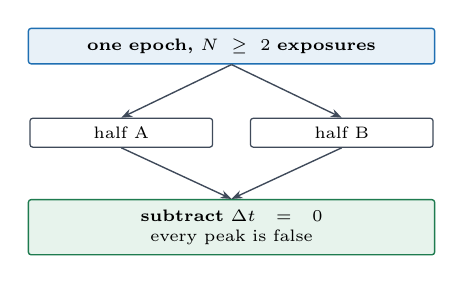
\begin{tikzpicture}[font=\fontsize{6}{7.2}\selectfont,
    b/.style={draw=accent,line width=0.5pt,fill=accent2,rounded corners=1pt,
      align=center,inner sep=1.3mm,text width=4.9cm},
    g/.style={draw=good,line width=0.5pt,fill=good2,rounded corners=1pt,
      align=center,inner sep=1.3mm,text width=4.9cm},
    s/.style={draw=slate,fill=white,line width=0.45pt,rounded corners=1pt,
      align=center,inner sep=1.1mm,text width=2.1cm},
    ar/.style={-{Stealth[length=1.4mm]},draw=slate,line width=0.5pt}]
    \node[b] (e) at (2.65,3.15) {\textbf{one epoch, $N\ge2$ exposures}};
    \node[s] (h1) at (1.25,2.05) {half A};
    \node[s] (h2) at (4.05,2.05) {half B};
    \node[g] (sub) at (2.65,0.85) {\textbf{subtract} $\Delta t=0$\\ every peak is false};
    \draw[ar] (e.south) -- (h1.north); \draw[ar] (e.south) -- (h2.north);
    \draw[ar] (h1.south) -- (sub.north); \draw[ar] (h2.south) -- (sub.north);
  \end{tikzpicture}
  \figcap{The null test needs no truth table: the physics guarantees the answer is zero.}
}
\end{frame}

% ============================================ 16. INJECTION-RECOVERY ======
\begin{frame}
\kicker{Validation II · completeness}
\frametitle{Plant 12\,240 sources and count what comes back}
\lead{Recovery only counts if the source is found within 1.5 pixels \emph{and} classified as the
kind we planted.}

\twocol{7.0cm}{%
  \centering
  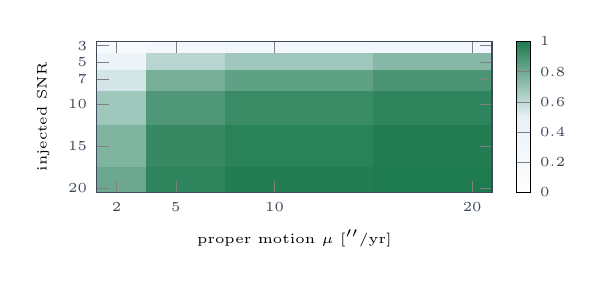
\begin{tikzpicture}[font=\fontsize{5.8}{7}\selectfont]
    \begin{axis}[width=6.6cm,height=3.5cm,
      view={0}{90},colormap={rec}{color=(white) color=(accent2) color=(good)},
      colorbar,colorbar style={font=\fontsize{5}{6},width=0.18cm},
      xlabel={proper motion $\mu$ [$''$/yr]},ylabel={injected SNR},
      xlabel style={font=\fontsize{5.4}{6.6}\selectfont},
      ylabel style={font=\fontsize{5.4}{6.6}\selectfont},
      xtick={2,5,10,20},ytick={3,5,7,10,15,20},
      xmin=1,xmax=21,ymin=2.5,ymax=20.5,
      tick label style={font=\fontsize{5}{6}\selectfont,text=slate},
      axis line style={slate},point meta min=0,point meta max=1]
      \addplot[matrix plot,mesh/cols=4,mesh/rows=6,point meta=explicit] coordinates {
        (2,3)[0.18] (5,3)[0.24] (10,3)[0.28] (20,3)[0.32]
        (2,5)[0.42] (5,5)[0.62] (10,5)[0.68] (20,5)[0.74]
        (2,7)[0.55] (5,7)[0.78] (10,7)[0.84] (20,7)[0.89]
        (2,10)[0.68] (5,10)[0.88] (10,10)[0.93] (20,10)[0.96]
        (2,15)[0.76] (5,15)[0.94] (10,15)[0.97] (20,15)[0.99]
        (2,20)[0.81] (5,20)[0.96] (10,20)[0.99] (20,20)[1.00]
      };
    \end{axis}
  \end{tikzpicture}
  \figcap{Recovery rises with both signal-to-noise and proper motion; slow movers are the hard
  case.}
}{%
  \begin{itemize}\setlength{\itemsep}{0.5mm}
    \item \textbf{96.7\%} of brightening transients recovered; \textbf{95.3\%} of fading ones.
    \item Only \textbf{56.0\%} of moving dipoles: below $2''$/yr the lobes overlap inside the PSF.
    \item Overall \textbf{69.3\%} strictly recovered — versus 0.2\% before Decision A.
  \end{itemize}
}
\end{frame}

\begin{frame}
\kicker{Confusers · the solar system}
\frametitle{Asteroids move faster than anything else in the frame}
\lead{An asteroid vacates its coordinates within hours, leaving a monopole that mimics a flare.
It has to be identified, not vetoed by hand.}

\figureblock{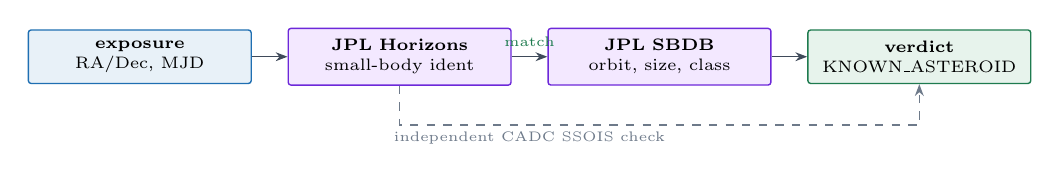
\begin{tikzpicture}[font=\fontsize{6}{7.2}\selectfont,
  b/.style={draw=accent,line width=0.5pt,fill=accent2,rounded corners=1pt,
    align=center,inner sep=1.4mm,text width=2.55cm},
  p/.style={draw=purple,line width=0.5pt,fill=purple2,rounded corners=1pt,
    align=center,inner sep=1.4mm,text width=2.55cm},
  g/.style={draw=good,line width=0.5pt,fill=good2,rounded corners=1pt,
    align=center,inner sep=1.4mm,text width=2.55cm},
  ar/.style={-{Stealth[length=1.5mm]},draw=slate,line width=0.5pt}]
  \node[b] (e) at (1.45,1.45) {\textbf{exposure}\\ RA/Dec, MJD};
  \node[p] (h) at (4.75,1.45) {\textbf{JPL Horizons}\\ small-body ident};
  \node[p] (s) at (8.05,1.45) {\textbf{JPL SBDB}\\ orbit, size, class};
  \node[g] (v) at (11.35,1.45) {\textbf{verdict}\\ KNOWN\_ASTEROID};
  \draw[ar] (e) -- (h); \draw[ar] (h) -- node[above,font=\fontsize{5.4}{6.6}\selectfont,text=good]{match} (s);
  \draw[ar] (s) -- (v);
  \draw[ar,dashed,draw=muted] (h.south) -- ++(0,-0.5) -| (v.south);
  \node[text=muted,font=\fontsize{5.4}{6.6}\selectfont] at (6.4,0.42) {independent CADC SSOIS check};
\end{tikzpicture}
\figcap{Every exposure timestamp is queried against JPL, enriched with orbital data and
cross-checked geometrically against an independent archive.}}

\vspace{0.2mm}
\begin{itemize}\setlength{\itemsep}{0.3mm}
  \item A 25-second time-box guards the call: if JPL is unreachable the card says ``asteroid check
        unavailable'' rather than silently defaulting to candidate.
\end{itemize}
\end{frame}

\begin{frame}
\kicker{Theory V · identity}
\frametitle{Six verdicts, and one of them means ``unknown''}
\lead{Catalogue matching is where a detection becomes an identity. The interesting cases are the
ones that survive every catalogue.}

\twocol{6.7cm}{%
  \begin{itemize}\setlength{\itemsep}{0.4mm}
    \item Gaia coordinates are propagated to the exposure epoch: Barnard's Star moves 94\arcsec\
          in 9.8 years.
    \item Match radii scale with brightness — 10\arcsec\ for faint stars, 120\arcsec\ for bright
          ones, plus a 180\arcsec\ halo veto.
    \item The result: 99 of 109 detections explained, 10 left for follow-up.
  \end{itemize}
}{%
  \centering
  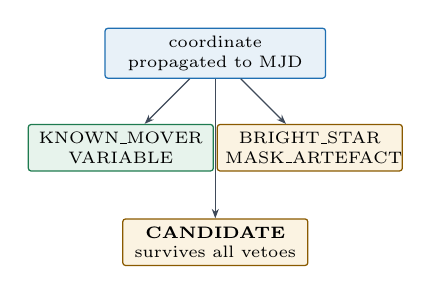
\begin{tikzpicture}[font=\fontsize{5.8}{7}\selectfont,
    k/.style={draw=good,line width=0.45pt,fill=good2,rounded corners=1pt,
      align=center,inner sep=1mm,text width=2.15cm},
    w/.style={draw=warn,line width=0.45pt,fill=warn2,rounded corners=1pt,
      align=center,inner sep=1mm,text width=2.15cm},
    ar/.style={-{Stealth[length=1.2mm]},draw=slate,line width=0.45pt}]
    \node[draw=accent,line width=0.45pt,fill=accent2,rounded corners=1pt,
      align=center,inner sep=1mm,text width=2.6cm] (in) at (2.4,3.10)
      {coordinate\\ propagated to MJD};
    \node[k] (a) at (1.20,1.90) {KNOWN\_MOVER\\ VARIABLE};
    \node[w] (b) at (3.60,1.90) {BRIGHT\_STAR\\ MASK\_ARTEFACT};
    \node[w] (c) at (2.4,0.70) {\textbf{CANDIDATE}\\ survives all vetoes};
    \draw[ar] (in) -- (a); \draw[ar] (in) -- (b); \draw[ar] (in) -- (c);
  \end{tikzpicture}
  \figcap{Six categories, one decision tree. Only the residual class is reported as a candidate.}
}
\end{frame}

\begin{frame}
\kicker{Machine learning, used honestly}
\frametitle{A ranking aid that never overrides the catalogues}
\lead{The classifier sorts candidates for a human; it does not decide identity. Its headline
score is inflated by synthetic dipoles, and we say so.}

\twocol{6.6cm}{%
  \centering
  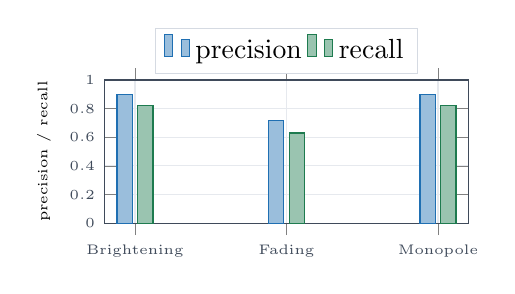
\begin{tikzpicture}[font=\fontsize{5.6}{6.8}\selectfont]
    \begin{axis}[width=6.2cm,height=3.4cm,ybar,bar width=5.5pt,ymin=0,ymax=1.0,
      ylabel={precision / recall},ylabel style={font=\fontsize{5.4}{6.6}\selectfont},
      symbolic x coords={{Brightening},{Fading},{Monopole}},
      xtick=data,tick label style={font=\fontsize{5}{6}\selectfont,text=slate},
      axis line style={slate},grid=major,grid style={rule!60},
      legend style={font=\fontsize{4.8}{5.8},draw=rule,at={(0.5,1.04)},anchor=south,
        legend columns=2}]
      \addplot[fill=accent!45,draw=accent] coordinates {
        ({Brightening},0.90) ({Fading},0.72) ({Monopole},0.90)};
      \addlegendentry{precision}
      \addplot[fill=good!45,draw=good] coordinates {
        ({Brightening},0.82) ({Fading},0.63) ({Monopole},0.82)};
      \addlegendentry{recall}
    \end{axis}
  \end{tikzpicture}
  \figcap{Held-out skill, reported by kind rather than as one flattering number.}
}{%
  \begin{itemize}\setlength{\itemsep}{0.45mm}
    \item 22 engineered features (SNR, $\chi^2$, ellipticity, FWHM ratio, masked fraction) feed a
          gradient-boosted classifier trained on 12\,150 labels.
    \item Isotonic calibration turns the score into a posterior, validated by field-wise
          GroupKFold plus four held-out fields.
    \item Every score ships with its top-three reasons, and public votes retrain the next model.
  \end{itemize}
}
\end{frame}

\begin{frame}
\kicker{Combining evidence}
\frametitle{Five independent streams, one believability score}
\lead{A single metric — significance, or a network's confidence — is not enough to justify
expensive follow-up.}

\figureblock{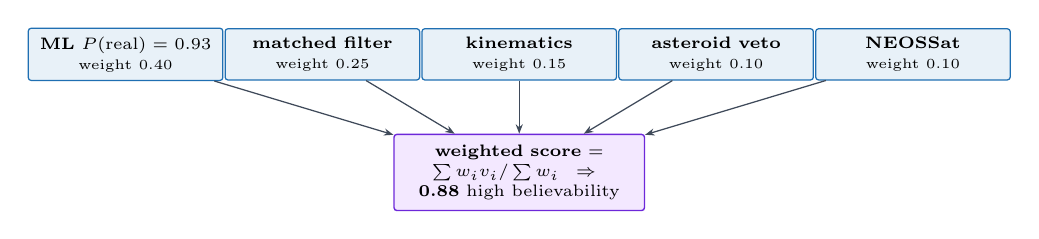
\begin{tikzpicture}[font=\fontsize{5.9}{7.1}\selectfont,
  b/.style={draw=accent,line width=0.45pt,fill=accent2,rounded corners=1pt,
    align=center,inner sep=1.1mm,text width=2.25cm},
  p/.style={draw=purple,line width=0.5pt,fill=purple2,rounded corners=1pt,
    align=center,inner sep=1.4mm,text width=2.9cm},
  ar/.style={-{Stealth[length=1.2mm]},draw=slate,line width=0.45pt}]
  \node[b] (a) at (1.25,2.35) {\textbf{ML} $P(\mathrm{real})=0.93$\\ \fontsize{5.2}{6.4}\selectfont weight 0.40};
  \node[b] (b) at (3.75,2.35) {\textbf{matched filter}\\ \fontsize{5.2}{6.4}\selectfont weight 0.25};
  \node[b] (c) at (6.25,2.35) {\textbf{kinematics}\\ \fontsize{5.2}{6.4}\selectfont weight 0.15};
  \node[b] (d) at (8.75,2.35) {\textbf{asteroid veto}\\ \fontsize{5.2}{6.4}\selectfont weight 0.10};
  \node[b] (e) at (11.25,2.35) {\textbf{NEOSSat}\\ \fontsize{5.2}{6.4}\selectfont weight 0.10};
  \node[p] (f) at (6.25,0.85) {\textbf{weighted score} $=\sum w_i v_i/\sum w_i$ $\;\Rightarrow\;$
    \textbf{0.88} high believability};
  \draw[ar] (a) -- (f); \draw[ar] (b) -- (f); \draw[ar] (c) -- (f); \draw[ar] (d) -- (f);
  \draw[ar] (e) -- (f);
\end{tikzpicture}
\figcap{Every stream shows its weight and a plain-language reason in the interface; a stream that
is unavailable reports a null weight instead of penalising the candidate.}}

\vspace{0.2mm}
\begin{itemize}\setlength{\itemsep}{0.3mm}
  \item The score ranks candidates. It never promotes one past a catalogue match.
\end{itemize}
\end{frame}

\begin{frame}
\kicker{Time domain}
\frametitle{At the ecliptic pole, the same star is seen 20\,800 times}
\lead{SPHEREx rolls between orbits, so a star lands on different pixels — and at different
wavelengths — on every visit.}

\twocol{6.0cm}{%
  \centering
  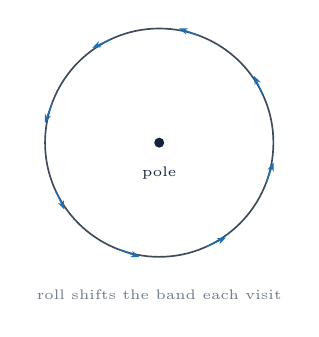
\begin{tikzpicture}[font=\fontsize{5.6}{6.8}\selectfont]
    \draw[slate,line width=0.6pt] (2.2,1.9) circle (1.45);
    \fill[ink] (2.2,1.9) circle (1.8pt);
    \node[text=ink,font=\fontsize{5}{6}\selectfont,anchor=north] at (2.2,1.72) {pole};
    \foreach \ang in {25,70,115,160,205,250,295,340}{
      \draw[-{Stealth[length=1.1mm]},accent,line width=0.5pt]
        ({2.2+1.45*cos(\ang)},{1.9+1.45*sin(\ang)}) -- ++({-0.26*sin(\ang)},{0.26*cos(\ang)});
    }
    \node[text=muted,font=\fontsize{5.2}{6.4}\selectfont,anchor=north] at (2.2,0.15)
      {roll shifts the band each visit};
  \end{tikzpicture}
  \figcap{Polar geometry: the field sweeps past the pole on every orbit.}
}{%
  \begin{itemize}\setlength{\itemsep}{0.4mm}
    \item Raw photometry swings by tens of percent purely because the filter angle changed.
    \item Dividing each visit by the star's own spectrum removes the artefact and leaves the true
          pulsation.
    \item On 78 NEP visits the pipeline flagged exactly one of six stars as variable — the same
          star Gaia DR3 independently lists.
  \end{itemize}
}
\end{frame}

% ================================================ 22. SPECTROSCOPY ========
\begin{frame}
\kicker{Theory VI · colour}
\frametitle{102 bands, read as a spectrum}
\lead{Because every pixel knows its wavelength, a cut-out becomes a low-resolution spectrum.}

\figureblock{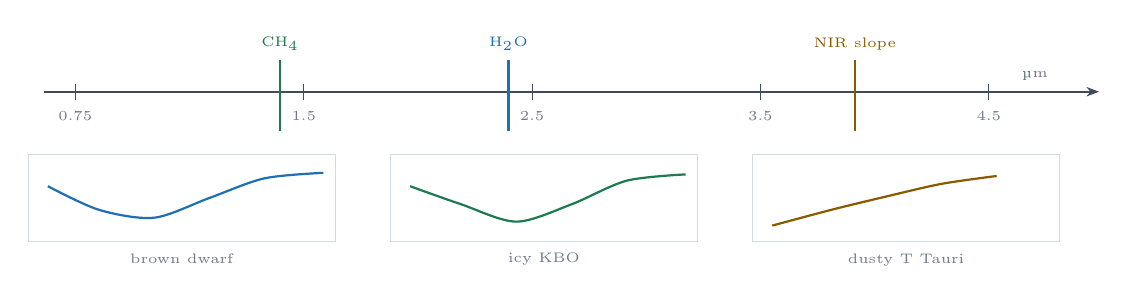
\begin{tikzpicture}[font=\fontsize{5.9}{7.1}\selectfont]
  \draw[-{Stealth[length=1.6mm]},draw=slate,line width=0.6pt] (0.2,2.05) -- (13.6,2.05);
  \foreach \x/\lab in {0.6/0.75, 3.5/1.5, 6.4/2.5, 9.3/3.5, 12.2/4.5}{
    \draw[slate,line width=0.4pt] (\x,1.95) -- (\x,2.15);
    \node[anchor=north,text=muted,font=\fontsize{5.2}{6.4}\selectfont] at (\x,1.92) {\lab};
  }
  \node[anchor=west,text=muted,font=\fontsize{5.4}{6.6}\selectfont] at (12.5,2.25) {µm};
  % band markers
  \foreach \x/\lab/\col in {3.2/{CH$_4$}/good, 6.1/{H$_2$O}/accent, 10.5/{NIR slope}/warn}{
    \draw[\col,line width=0.9pt] (\x,1.55) -- (\x,2.45);
    \node[anchor=south,text=\col,font=\fontsize{5.4}{6.6}\selectfont] at (\x,2.45) {\lab};
  }
  % template curves
  \foreach \dx/\col in {0/accent, 4.6/good, 9.2/warn}{
    \draw[rule,line width=0.35pt] (\dx,0.15) rectangle (\dx+3.9,1.25);
  }
  \draw[accent,line width=0.8pt] plot[smooth] coordinates {(0.25,0.85) (0.9,0.55) (1.6,0.45)
    (2.3,0.70) (3.0,0.95) (3.75,1.02)};
  \draw[good,line width=0.8pt] plot[smooth] coordinates {(4.85,0.85) (5.5,0.62) (6.2,0.40)
    (6.9,0.62) (7.6,0.92) (8.35,1.00)};
  \draw[warn,line width=0.8pt] plot[smooth] coordinates {(9.45,0.35) (10.2,0.55) (10.9,0.72)
    (11.6,0.88) (12.3,0.98)};
  \node[anchor=north,text=muted,font=\fontsize{5}{6}\selectfont] at (1.95,0.12) {brown dwarf};
  \node[anchor=north,text=muted,font=\fontsize{5}{6}\selectfont] at (6.55,0.12) {icy KBO};
  \node[anchor=north,text=muted,font=\fontsize{5}{6}\selectfont] at (11.15,0.12) {dusty T Tauri};
\end{tikzpicture}
\figcap{Three indices — methane, water and the near-infrared slope — separate brown dwarfs, icy
bodies and young stars.}}
\vspace{-0.6mm}
\begin{itemize}\setlength{\itemsep}{0.0mm}
  \item The classifier refuses to answer with fewer than 30 usable bands; below that it reports raw
        fluxes instead of guessing a label.
\end{itemize}
\end{frame}

\begin{frame}
\kicker{Implementation I · backend}
\frametitle{One FastAPI service, seven routers, one job pool}
\lead{The science stays in modules; the web layer only orchestrates.}

\figureblock{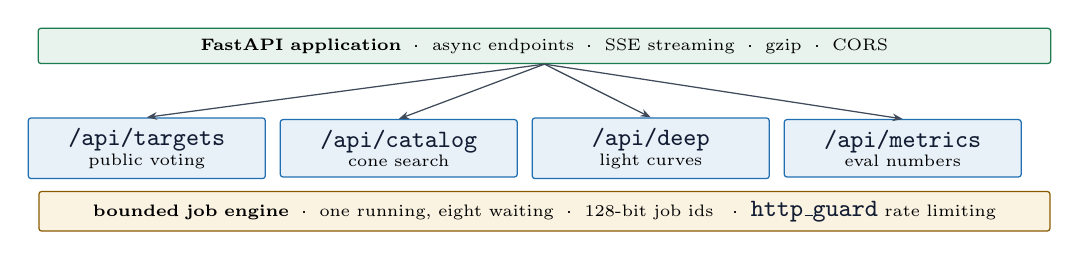
\begin{tikzpicture}[font=\fontsize{5.9}{7.1}\selectfont,
  b/.style={draw=accent,line width=0.45pt,fill=accent2,rounded corners=1pt,
    align=center,inner sep=1.3mm,text width=2.75cm},
  g/.style={draw=good,line width=0.45pt,fill=good2,rounded corners=1pt,
    align=center,inner sep=1.3mm,text width=3.4cm},
  ar/.style={-{Stealth[length=1.3mm]},draw=slate,line width=0.45pt}]
  \node[g,text width=12.6cm] (api) at (6.6,2.45)
    {\textbf{FastAPI application} \;·\; async endpoints \;·\; SSE streaming \;·\; gzip \;·\; CORS};
  \node[b] (r1) at (1.55,1.15) {\code{/api/targets}\\ public voting};
  \node[b] (r2) at (4.75,1.15) {\code{/api/catalog}\\ cone search};
  \node[b] (r3) at (7.95,1.15) {\code{/api/deep}\\ light curves};
  \node[b] (r4) at (11.15,1.15) {\code{/api/metrics}\\ eval numbers};
  \draw[ar] (api.south) -- (r1.north); \draw[ar] (api.south) -- (r2.north);
  \draw[ar] (api.south) -- (r3.north); \draw[ar] (api.south) -- (r4.north);
  \node[draw=warn,line width=0.45pt,fill=warn2,rounded corners=1pt,
    align=center,inner sep=1.2mm,text width=12.6cm] (job) at (6.6,0.35)
    {\textbf{bounded job engine} \;·\; one running, eight waiting \;·\; 128-bit job ids \;
     ·\; \code{http\_guard} rate limiting};
\end{tikzpicture}
\figcap{Routers stay thin: they validate input, enqueue work and stream results. Heavy archive
fetches never block a cached read.}}

\vspace{0.2mm}
\begin{itemize}\setlength{\itemsep}{0.3mm}
  \item Structured JSON logs carry a correlation id, so one request can be followed from the
        router to the archive call.
\end{itemize}
\end{frame}

\begin{frame}
\kicker{Implementation II · deployment}
\frametitle{Reads and live work run in different services}
\lead{A cached read must never queue behind a forty-second archive download.}

\figureblock{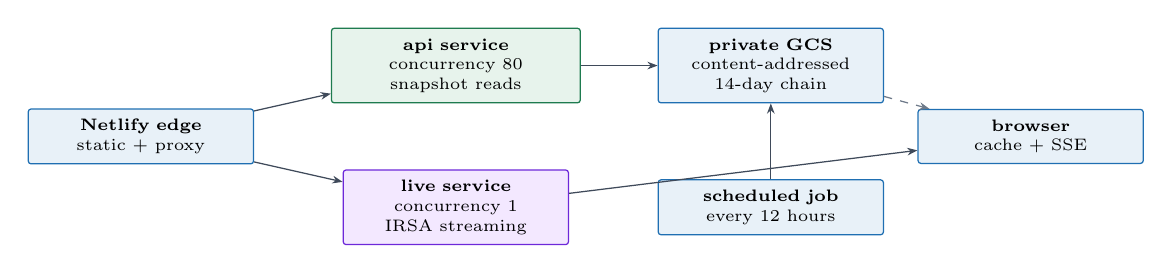
\begin{tikzpicture}[font=\fontsize{5.9}{7.1}\selectfont,
  b/.style={draw=accent,line width=0.45pt,fill=accent2,rounded corners=1pt,
    align=center,inner sep=1.3mm,text width=2.6cm},
  g/.style={draw=good,line width=0.45pt,fill=good2,rounded corners=1pt,
    align=center,inner sep=1.3mm,text width=2.9cm},
  p/.style={draw=purple,line width=0.45pt,fill=purple2,rounded corners=1pt,
    align=center,inner sep=1.3mm,text width=2.6cm},
  ar/.style={-{Stealth[length=1.3mm]},draw=slate,line width=0.45pt}]
  \node[b] (edge) at (1.55,1.55) {\textbf{Netlify edge}\\ static + proxy};
  \node[g] (api) at (5.55,2.45) {\textbf{api service}\\ concurrency 80\\ snapshot reads};
  \node[p] (live) at (5.55,0.65) {\textbf{live service}\\ concurrency 1\\ IRSA streaming};
  \node[b] (gcs) at (9.55,2.45) {\textbf{private GCS}\\ content-addressed\\ 14-day chain};
  \node[b] (job) at (9.55,0.65) {\textbf{scheduled job}\\ every 12 hours};
  \node[b] (cdn) at (12.85,1.55) {\textbf{browser}\\ cache + SSE};
  \draw[ar] (edge) -- (api); \draw[ar] (edge) -- (live);
  \draw[ar] (api) -- (gcs); \draw[ar] (job) -- (gcs);
  \draw[ar,dashed,draw=muted] (gcs) -- (cdn); \draw[ar] (live) -- (cdn);
\end{tikzpicture}
\figcap{Two services, one image: the api answers from snapshots in milliseconds, the live service
absorbs long archive calls, and a scheduled job refreshes the snapshots.}}

\vspace{0.2mm}
\begin{itemize}\setlength{\itemsep}{0.3mm}
  \item A 21-point security review closed with signed proxy tokens, non-root containers and
        hashed lock files.
\end{itemize}
\end{frame}

\begin{frame}
\kicker{Implementation III · interface}
\frametitle{A mission console in the browser, no build step}
\lead{The interface is plain HTML, CSS and JavaScript: 7\,611 lines that run without a toolchain.}

\twocol{6.5cm}{%
  \begin{itemize}\setlength{\itemsep}{0.4mm}
    \item A NASA-style dark console: toolbar, telemetry strip, four key numbers, split viewer and
          verdict card.
    \item A two-stage canvas engine clips the 0.5–99.5 percentile, maps a 256-level colour ramp
          offscreen, then composites five vector overlays.
    \item A service worker keeps recent snapshots offline; history holds 200\,MB in the browser.
  \end{itemize}
}{%
  \centering
  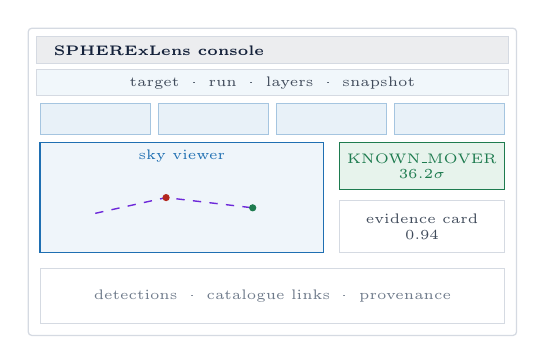
\begin{tikzpicture}[font=\fontsize{5.2}{6.4}\selectfont]
    \draw[rule,line width=0.45pt,fill=white,rounded corners=1.2pt] (0,0) rectangle (6.2,3.9);
    \draw[rule,fill=ink!8] (0.1,3.45) rectangle (6.1,3.8);
    \node[anchor=west,text=ink,font=\fontsize{5}{6}\selectfont\bfseries] at (0.2,3.62)
      {SPHERExLens console};
    \draw[rule,fill=accent2!60] (0.1,3.05) rectangle (6.1,3.38);
    \node[text=slate,font=\fontsize{4.8}{5.8}\selectfont] at (3.1,3.21)
      {target \;·\; run \;·\; layers \;·\; snapshot};
    \foreach \i in {0,1,2,3}{
      \draw[accent!40,fill=accent2,line width=0.3pt] (0.15+\i*1.50,2.55) rectangle (1.55+\i*1.50,2.95);
    }
    \draw[accent,line width=0.45pt,fill=accent2!70] (0.15,1.05) rectangle (3.75,2.45);
    \node[text=accent,font=\fontsize{4.8}{5.8}\selectfont] at (1.95,2.28) {sky viewer};
    \draw[purple,line width=0.5pt,dashed] (0.85,1.55) -- (1.75,1.75) -- (2.85,1.62);
    \fill[bad] (1.75,1.75) circle (1.3pt); \fill[good] (2.85,1.62) circle (1.3pt);
    \draw[good,line width=0.4pt,fill=good2] (3.95,1.85) rectangle (6.05,2.45);
    \node[text=good,font=\fontsize{4.6}{5.6}\selectfont,align=center] at (5.0,2.15)
      {KNOWN\_MOVER\\ $36.2\sigma$};
    \draw[rule,line width=0.3pt,fill=white] (3.95,1.05) rectangle (6.05,1.72);
    \node[text=slate,font=\fontsize{4.6}{5.6}\selectfont,align=center] at (5.0,1.38)
      {evidence card\\ 0.94};
    \draw[rule,line width=0.3pt,fill=white] (0.15,0.15) rectangle (6.05,0.85);
    \node[text=muted,font=\fontsize{4.6}{5.6}\selectfont,align=center] at (3.1,0.50)
      {detections \;·\; catalogue links \;·\; provenance};
  \end{tikzpicture}
  \figcap{Wireframe of the console: viewer and verdict dominate, diagnostics sit underneath.}
}
\end{frame}

\begin{frame}
\kicker{Results · the census}
\frametitle{Eighteen fields, 109 detections, 99 explained}
\lead{Detection count is not discovery count: most of what survives subtraction is already in a
catalogue.}

\twocol{7.0cm}{%
  \centering
  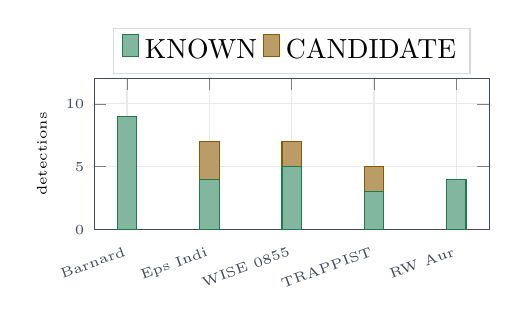
\begin{tikzpicture}[font=\fontsize{5.6}{6.8}\selectfont]
    \begin{axis}[width=6.6cm,height=3.5cm,ybar stacked,bar width=7pt,ymin=0,ymax=12,
      ylabel={detections},ylabel style={font=\fontsize{5.4}{6.6}\selectfont},
      symbolic x coords={{Barnard},{Eps Indi},{WISE 0855},{TRAPPIST},{RW Aur}},
      xtick=data,tick label style={font=\fontsize{4.8}{5.8}\selectfont,text=slate},
      xticklabel style={rotate=20,anchor=north east,yshift=-0.6mm},
      axis line style={slate},grid=major,grid style={rule!60},
      legend style={font=\fontsize{4.8}{5.8},draw=rule,at={(0.5,1.03)},anchor=south,
        legend columns=2}]
      \addplot[fill=good!55,draw=good] coordinates {
        ({Barnard},9) ({Eps Indi},4) ({WISE 0855},5) ({TRAPPIST},3) ({RW Aur},4)};
      \addlegendentry{KNOWN}
      \addplot[fill=warn!60,draw=warn] coordinates {
        ({Barnard},0) ({Eps Indi},3) ({WISE 0855},2) ({TRAPPIST},2) ({RW Aur},0)};
      \addlegendentry{CANDIDATE}
    \end{axis}
  \end{tikzpicture}
  \figcap{Five brief targets: 35 detections, 7 of them unexplained.}
}{%
  \begin{itemize}\setlength{\itemsep}{0.45mm}
    \item 109 detections across 18 fields and 246 cut-outs: \textbf{99 KNOWN} (91\%) and
          \textbf{10 CANDIDATE} (9\%).
    \item Sirius, M31, M104, M1 and Barnard's Star are fully explained.
    \item Two fields yield nothing: M42 is a null sky, and Sgr\,A* has no band shared by both
          epochs.
  \end{itemize}
}
\end{frame}


% ============================================ 27. RESULTS II ==============
\begin{frame}
\kicker{Results · the residuals}
\frametitle{Ten candidates, five fields, one caveat}
\lead{``Candidate'' means unexplained by Gaia, WISE, VSX or NEOWISE — not a claimed discovery.}

\figureblock{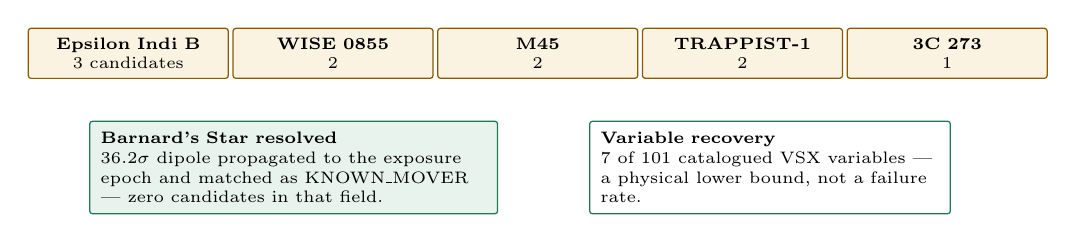
\begin{tikzpicture}[font=\fontsize{5.9}{7.1}\selectfont,
  b/.style={draw=warn,line width=0.45pt,fill=warn2,rounded corners=1pt,
    align=center,inner sep=1.2mm,text width=2.30cm},
  g/.style={draw=good,line width=0.45pt,fill=good2,rounded corners=1pt,
    align=left,inner sep=1.4mm,text width=4.9cm}]
  \node[b] (a) at (1.45,2.30) {\textbf{Epsilon Indi B}\\ 3 candidates};
  \node[b] (b) at (4.05,2.30) {\textbf{WISE 0855}\\ 2};
  \node[b] (c) at (6.65,2.30) {\textbf{M45}\\ 2};
  \node[b] (d) at (9.25,2.30) {\textbf{TRAPPIST-1}\\ 2};
  \node[b] (e) at (11.85,2.30) {\textbf{3C 273}\\ 1};
  \node[g] (f) at (3.55,0.85) {\textbf{Barnard's Star resolved}\\ $36.2\sigma$ dipole propagated
    to the exposure epoch and matched as KNOWN\_MOVER — zero candidates in that field.};
  \node[draw=good,line width=0.45pt,fill=white,rounded corners=1pt,
    align=left,inner sep=1.4mm,text width=4.3cm] (h) at (9.6,0.85)
    {\textbf{Variable recovery}\\ 7 of 101 catalogued VSX variables — a physical lower bound,
      not a failure rate.};
\end{tikzpicture}
\figcap{All ten residuals sit in five fields. Epoch propagation is what converts Barnard's Star
from an unexplained candidate into a catalogue match.}}

\vspace{0.2mm}
\begin{itemize}\setlength{\itemsep}{0.3mm}
  \item Faint infrared excesses beyond Gaia and WISE limits are exactly what SPHEREx was built to
        find — and exactly what needs follow-up.
\end{itemize}
\end{frame}

% ================================================ 28. LIVE DEMO ===========
\begin{frame}
\kicker{Live demonstration}
\frametitle{Six moves, one browser tab}
\lead{The deployed console is pre-loaded on Barnard's Star, so the demonstration is a guided walk
through real output.}

\figureblock{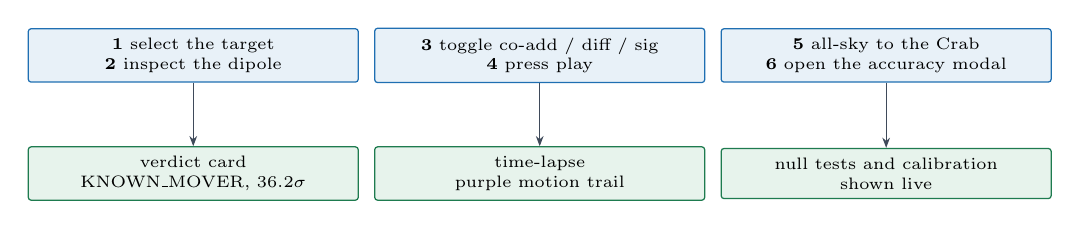
\begin{tikzpicture}[font=\fontsize{5.9}{7.1}\selectfont,
  b/.style={draw=accent,line width=0.45pt,fill=accent2,rounded corners=1pt,
    align=center,inner sep=1.2mm,text width=3.95cm},
  g/.style={draw=good,line width=0.45pt,fill=good2,rounded corners=1pt,
    align=center,inner sep=1.2mm,text width=3.95cm},
  ar/.style={-{Stealth[length=1.3mm]},draw=slate,line width=0.45pt}]
  \node[b] (m1) at (2.15,2.55) {\textbf{1} select the target\\ \textbf{2} inspect the dipole};
  \node[b] (m2) at (6.55,2.55) {\textbf{3} toggle co-add / diff / sig\\ \textbf{4} press play};
  \node[b] (m3) at (10.95,2.55) {\textbf{5} all-sky to the Crab\\ \textbf{6} open the accuracy modal};
  \node[g] (p1) at (2.15,1.05) {verdict card\\ KNOWN\_MOVER, $36.2\sigma$};
  \node[g] (p2) at (6.55,1.05) {time-lapse\\ purple motion trail};
  \node[g] (p3) at (10.95,1.05) {null tests and calibration\\ shown live};
  \draw[ar] (m1) -- (p1); \draw[ar] (m2) -- (p2); \draw[ar] (m3) -- (p3);
\end{tikzpicture}
\figcap{Moves run left to right: identify, animate, then audit. Every number shown comes from the
same pipeline that produced this deck.}}

\vspace{0.2mm}
\begin{itemize}\setlength{\itemsep}{0.3mm}
  \item If the venue network fails, a local copy and an offline service-worker cache keep the
        demonstration alive.
\end{itemize}
\end{frame}

% =============================================== 29. CONCLUSION ===========
\begin{frame}
\kicker{Conclusion}
\frametitle{Works, honest, and open}
\noindent
\begin{minipage}[t]{4.55cm}
  \kpi{good}{69.3\%}{WORKS}
  \vspace{0.6mm}{\fontsize{7.2}{9.2}\selectfont\color{ink}Strict recovery on 12\,240 injected sources.}
\end{minipage}\hfill
\begin{minipage}[t]{4.55cm}
  \kpi{accent}{1.66}{HONEST}
  \vspace{0.6mm}{\fontsize{7.2}{9.2}\selectfont\color{ink}False candidates per field in null tests.}
\end{minipage}\hfill
\begin{minipage}[t]{4.55cm}
  \kpi{purple}{21\,429}{OPEN}
  \vspace{0.6mm}{\fontsize{7.2}{9.2}\selectfont\color{ink}Runtime Python lines, all public and testable.}
\end{minipage}

\vspace{1.2mm}
\figureblock{
\begin{tikzpicture}[font=\fontsize{5.8}{7}\selectfont,
  b/.style={draw=rule,line width=0.45pt,fill=white,rounded corners=1pt,
    align=center,inner sep=1.1mm,text width=2.7cm}]
  \node[b] (a) at (1.55,1.55) {\textbf{next}\\ full-mission light curves};
  \node[b] (b) at (4.85,1.55) {\textbf{next}\\ GPU SFFT deconvolution};
  \node[b] (c) at (8.15,1.55) {\textbf{next}\\ active learning from votes};
  \node[b] (d) at (11.45,1.55) {\textbf{next}\\ IVOA cone-search federation};
  \node[anchor=west,font=\fontsize{7}{8.2}\selectfont\bfseries,text=accent] at (0.0,2.55)
    {Open horizons};
  \node[anchor=west,font=\fontsize{6.2}{7.4}\selectfont,text=muted] at (0.0,0.55)
    {Zackay, Ofek \& Gal-Yam 2016 (ZOGY) \;·\; Hu et al.\ 2022 (SFFT) \;·\; Gaia DR3 \;
     ·\; AllWISE / NEOWISE \;·\; NASA/IPAC IRSA SPHEREx DR1};
\end{tikzpicture}
\figcap{Everything in this talk is reproducible from public archives: 18 fields, 246 cut-outs and
one pipeline.}}
\end{frame}

\end{document}
